% Guide de démarrage rapide d'IPTV, édition française. Compiler dans ce
% dossier avec :
%   pdflatex IPTV-Quick-Start-fr.tex   (deux fois, pour la table des matières)
% (Les espaces avant « : ? ! » sont des espaces insécables écrites à la main.)
\newcommand{\GuideLang}{french}
\newcommand{\GuideTitle}{Guide de démarrage rapide}
\newcommand{\TipLabel}{Astuce.}
% Shared layout of the IPTV quick start guides (one file per language:
% IPTV-Quick-Start.tex, IPTV-Quick-Start-it.tex, ...). Each sets, before
% % Shared layout of the IPTV quick start guides (one file per language:
% IPTV-Quick-Start.tex, IPTV-Quick-Start-it.tex, ...). Each sets, before
% % Shared layout of the IPTV quick start guides (one file per language:
% IPTV-Quick-Start.tex, IPTV-Quick-Start-it.tex, ...). Each sets, before
% \input{preamble}:
%   \GuideLang   babel language (english, italian, spanish, french, ngerman, portuguese)
%   \GuideTitle  the guide's title, used on the cover, in headers and the PDF
%   \TipLabel    the word that starts a tip box ("Tip.")
% Build any of them with pdflatex, twice (for the table of contents).
\documentclass[11pt,a4paper]{article}

\usepackage[T1]{fontenc}
\usepackage[utf8]{inputenc}
% shorthands=off: no language-specific active characters (they would clash
% with tables and addresses); only hyphenation and "Contents" etc. change.
\usepackage[shorthands=off,\GuideLang]{babel}
\usepackage{lmodern}
\usepackage[scaled=0.92]{helvet}
\renewcommand{\familydefault}{\sfdefault}
\usepackage[margin=2.2cm,headheight=14pt]{geometry}
\usepackage{graphicx}
\usepackage[table]{xcolor}
\usepackage{booktabs}
\usepackage{tabularx}
\usepackage{xltabular}
\usepackage{enumitem}
\usepackage{titlesec}
\usepackage{fancyhdr}
\usepackage{pifont}
\usepackage{amssymb}
\usepackage[hidelinks]{hyperref}

\newcommand{\version}{0.12}
\definecolor{accent}{HTML}{1E6FD9}
\definecolor{dim}{HTML}{5F6673}
\definecolor{notebg}{HTML}{EEF4FC}
\definecolor{warnbg}{HTML}{FFF6E0}
\definecolor{tvred}{HTML}{D32F2F}
\definecolor{tvgreen}{HTML}{2E7D32}
\definecolor{tvyellow}{HTML}{C9A400}
\definecolor{tvblue}{HTML}{1565C0}

\hypersetup{pdftitle={IPTV -- \GuideTitle}, pdfauthor={IPTV project}}
\setlist{itemsep=2pt, topsep=4pt}
\setlength{\parindent}{0pt}
\setlength{\parskip}{6pt}
\renewcommand{\arraystretch}{1.25}

\titleformat{\section}{\Large\bfseries\color{accent}}{\thesection}{0.6em}{}
\titleformat{\subsection}{\large\bfseries}{\thesubsection}{0.6em}{}
\titlespacing*{\section}{0pt}{14pt}{6pt}
\titlespacing*{\subsection}{0pt}{10pt}{4pt}

\pagestyle{fancy}
\fancyhf{}
\fancyhead[L]{\small\color{dim}IPTV -- \GuideTitle}
\fancyhead[R]{\small\color{dim}github.com/vickdini/iptv}
\fancyfoot[C]{\small\color{dim}\thepage}
\renewcommand{\headrulewidth}{0.4pt}
\renewcommand{\sectionmark}[1]{\markboth{#1}{}}

% A key or button on a keyboard / remote.
\newcommand{\key}[1]{{\setlength{\fboxsep}{1.5pt}\fbox{\footnotesize\vphantom{Ay}#1}}}
% A coloured remote button.
\newcommand{\colorkey}[2]{\textcolor{#1}{\ding{108}}\,\textbf{#2}}
% Shaded boxes for tips and notes.
\newcommand{\tip}[1]{\par\noindent\colorbox{notebg}{\parbox{\dimexpr\linewidth-2\fboxsep}{\small\textbf{\TipLabel} #1}}\par}
\newcommand{\note}[1]{\par\noindent\colorbox{warnbg}{\parbox{\dimexpr\linewidth-2\fboxsep}{\small #1}}\par}
\newcommand{\menu}[1]{\textit{#1}}
\newcommand{\download}{\url{https://github.com/vickdini/iptv/releases/latest}}
% Key tables: \rowcolors{2}{gray!8}{white} then
% \begin{xltabular}{\linewidth}{@{}KX@{}} \keyshead{Key}{What it does} ... \bottomrule
\newcolumntype{K}{>{\raggedright\arraybackslash}p{5.4cm}}
\newcommand{\keyshead}[2]{\toprule \textbf{#1} & \textbf{#2} \\ \midrule}

% The cover: #1 subtitle, #2 "Version".
\newcommand{\cover}[2]{%
\begin{titlepage}
  \centering
  \vspace*{0.5cm}
  {\fontsize{40}{48}\selectfont\bfseries\color{accent} IPTV\par}
  \vspace{0.3cm}
  {\LARGE \GuideTitle\par}
  \vspace{0.3cm}
  {\large\color{dim} #1\par}
  \vspace{1cm}
  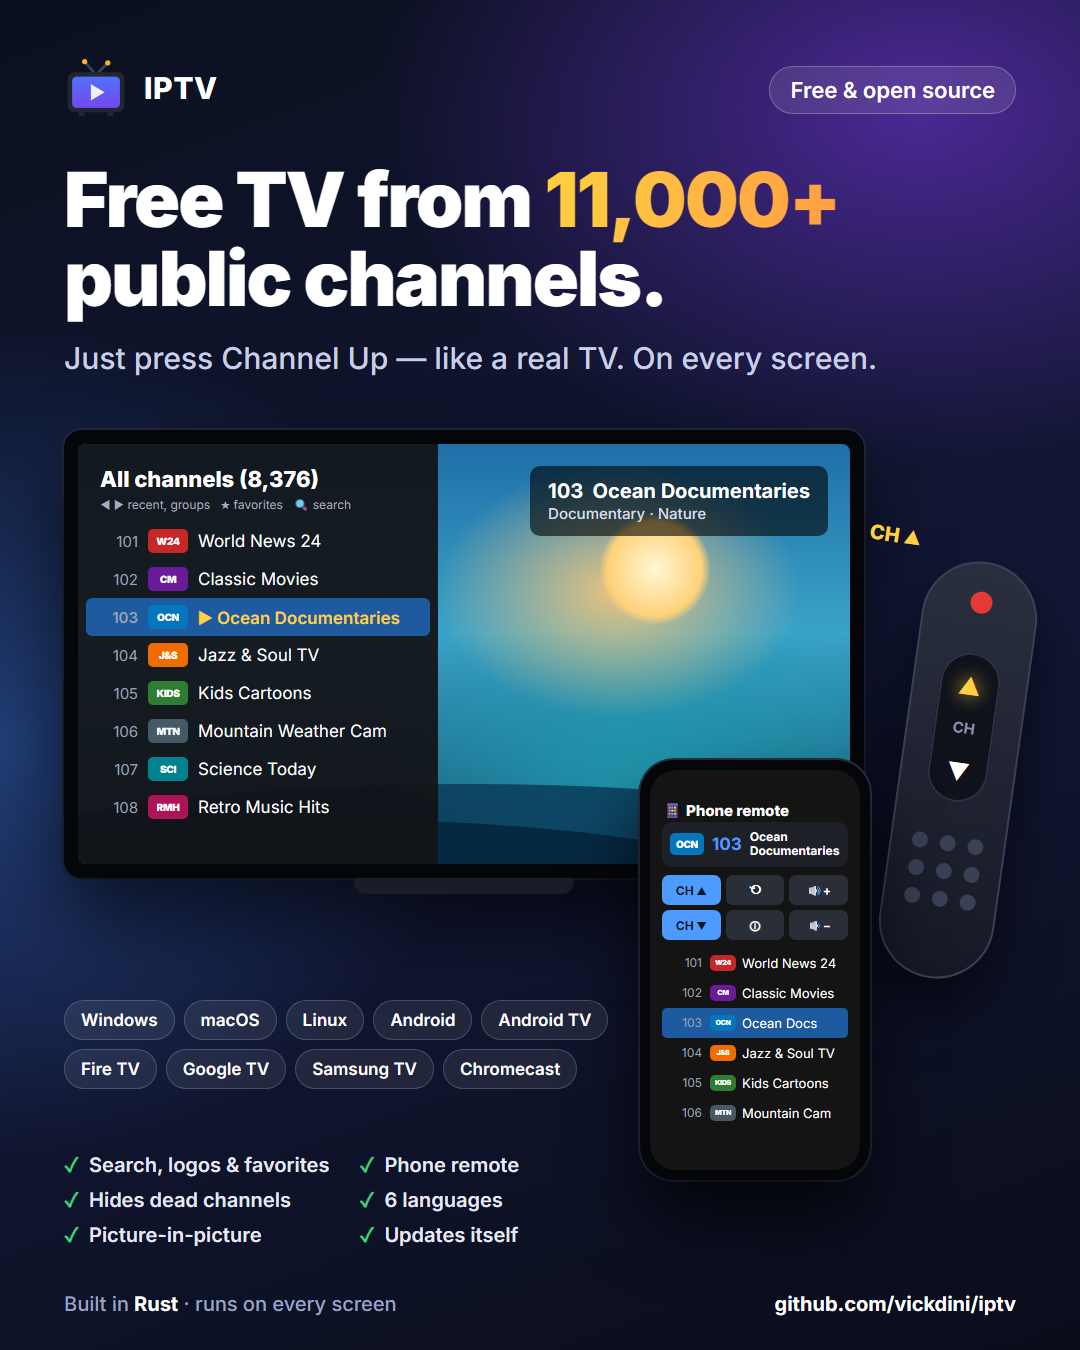
\includegraphics[width=0.52\textwidth]{../images/iptv-overview.png}\par
  \vfill
  {\large Windows \textbullet{} macOS \textbullet{} Linux \textbullet{} Android
   \textbullet{} Android TV \& Fire TV \textbullet{} Chromecast \textbullet{} Samsung TV\par}
  \vspace{0.5cm}
  {\color{dim} #2 \version{} \textbullet{} \url{https://github.com/vickdini/iptv}\par}
\end{titlepage}
\tableofcontents
\thispagestyle{fancy}}
:
%   \GuideLang   babel language (english, italian, spanish, french, ngerman, portuguese)
%   \GuideTitle  the guide's title, used on the cover, in headers and the PDF
%   \TipLabel    the word that starts a tip box ("Tip.")
% Build any of them with pdflatex, twice (for the table of contents).
\documentclass[11pt,a4paper]{article}

\usepackage[T1]{fontenc}
\usepackage[utf8]{inputenc}
% shorthands=off: no language-specific active characters (they would clash
% with tables and addresses); only hyphenation and "Contents" etc. change.
\usepackage[shorthands=off,\GuideLang]{babel}
\usepackage{lmodern}
\usepackage[scaled=0.92]{helvet}
\renewcommand{\familydefault}{\sfdefault}
\usepackage[margin=2.2cm,headheight=14pt]{geometry}
\usepackage{graphicx}
\usepackage[table]{xcolor}
\usepackage{booktabs}
\usepackage{tabularx}
\usepackage{xltabular}
\usepackage{enumitem}
\usepackage{titlesec}
\usepackage{fancyhdr}
\usepackage{pifont}
\usepackage{amssymb}
\usepackage[hidelinks]{hyperref}

\newcommand{\version}{0.12}
\definecolor{accent}{HTML}{1E6FD9}
\definecolor{dim}{HTML}{5F6673}
\definecolor{notebg}{HTML}{EEF4FC}
\definecolor{warnbg}{HTML}{FFF6E0}
\definecolor{tvred}{HTML}{D32F2F}
\definecolor{tvgreen}{HTML}{2E7D32}
\definecolor{tvyellow}{HTML}{C9A400}
\definecolor{tvblue}{HTML}{1565C0}

\hypersetup{pdftitle={IPTV -- \GuideTitle}, pdfauthor={IPTV project}}
\setlist{itemsep=2pt, topsep=4pt}
\setlength{\parindent}{0pt}
\setlength{\parskip}{6pt}
\renewcommand{\arraystretch}{1.25}

\titleformat{\section}{\Large\bfseries\color{accent}}{\thesection}{0.6em}{}
\titleformat{\subsection}{\large\bfseries}{\thesubsection}{0.6em}{}
\titlespacing*{\section}{0pt}{14pt}{6pt}
\titlespacing*{\subsection}{0pt}{10pt}{4pt}

\pagestyle{fancy}
\fancyhf{}
\fancyhead[L]{\small\color{dim}IPTV -- \GuideTitle}
\fancyhead[R]{\small\color{dim}github.com/vickdini/iptv}
\fancyfoot[C]{\small\color{dim}\thepage}
\renewcommand{\headrulewidth}{0.4pt}
\renewcommand{\sectionmark}[1]{\markboth{#1}{}}

% A key or button on a keyboard / remote.
\newcommand{\key}[1]{{\setlength{\fboxsep}{1.5pt}\fbox{\footnotesize\vphantom{Ay}#1}}}
% A coloured remote button.
\newcommand{\colorkey}[2]{\textcolor{#1}{\ding{108}}\,\textbf{#2}}
% Shaded boxes for tips and notes.
\newcommand{\tip}[1]{\par\noindent\colorbox{notebg}{\parbox{\dimexpr\linewidth-2\fboxsep}{\small\textbf{\TipLabel} #1}}\par}
\newcommand{\note}[1]{\par\noindent\colorbox{warnbg}{\parbox{\dimexpr\linewidth-2\fboxsep}{\small #1}}\par}
\newcommand{\menu}[1]{\textit{#1}}
\newcommand{\download}{\url{https://github.com/vickdini/iptv/releases/latest}}
% Key tables: \rowcolors{2}{gray!8}{white} then
% \begin{xltabular}{\linewidth}{@{}KX@{}} \keyshead{Key}{What it does} ... \bottomrule
\newcolumntype{K}{>{\raggedright\arraybackslash}p{5.4cm}}
\newcommand{\keyshead}[2]{\toprule \textbf{#1} & \textbf{#2} \\ \midrule}

% The cover: #1 subtitle, #2 "Version".
\newcommand{\cover}[2]{%
\begin{titlepage}
  \centering
  \vspace*{0.5cm}
  {\fontsize{40}{48}\selectfont\bfseries\color{accent} IPTV\par}
  \vspace{0.3cm}
  {\LARGE \GuideTitle\par}
  \vspace{0.3cm}
  {\large\color{dim} #1\par}
  \vspace{1cm}
  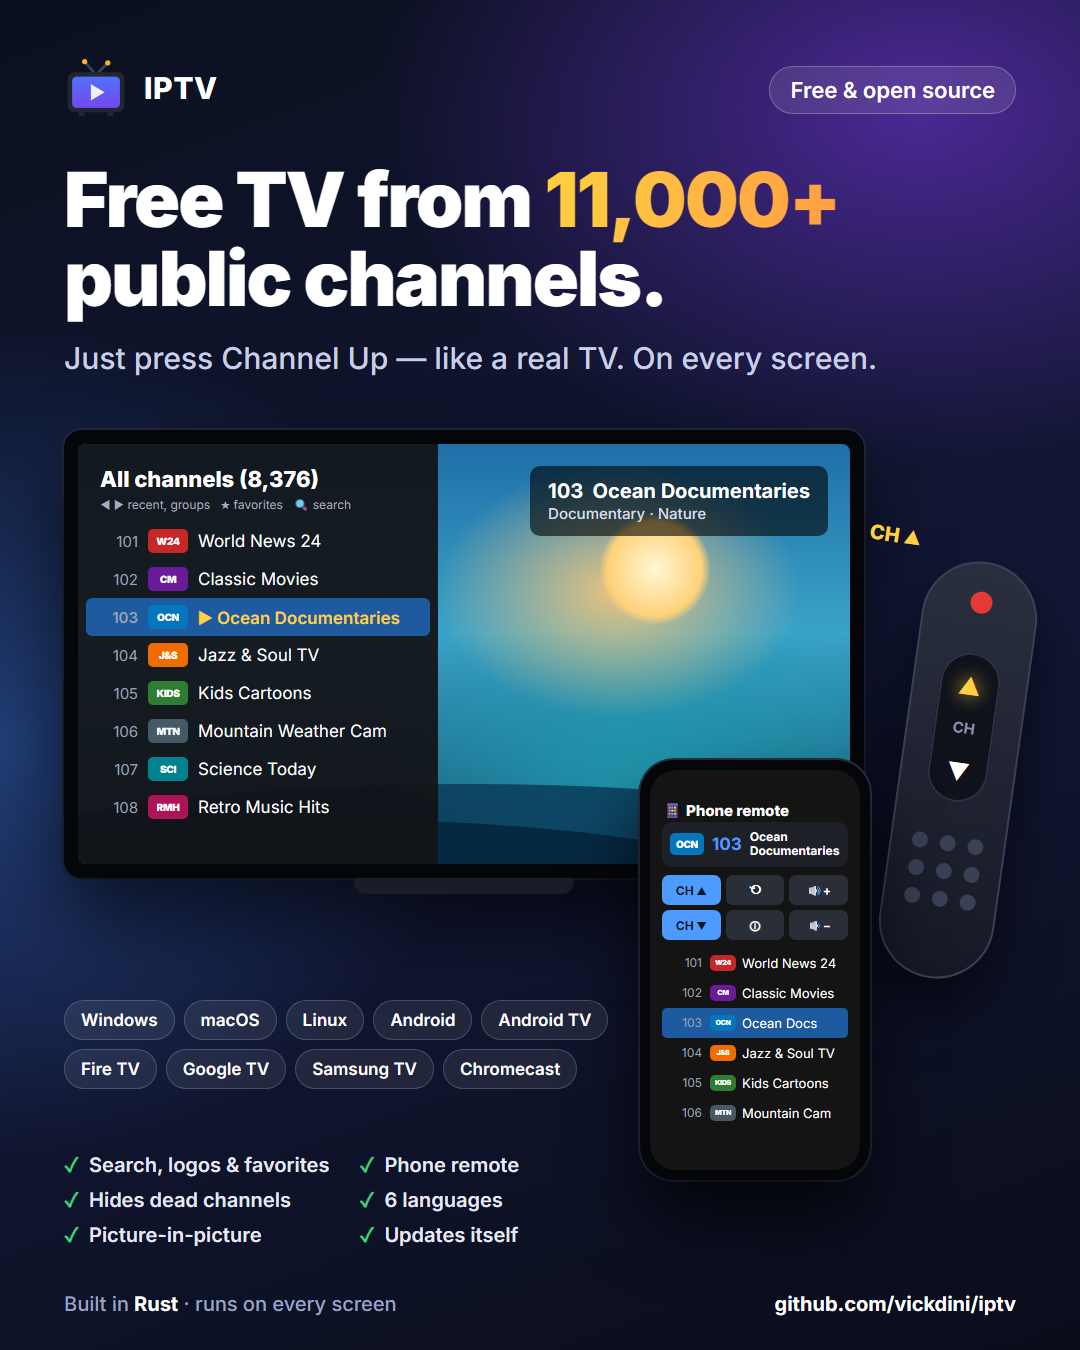
\includegraphics[width=0.52\textwidth]{../images/iptv-overview.png}\par
  \vfill
  {\large Windows \textbullet{} macOS \textbullet{} Linux \textbullet{} Android
   \textbullet{} Android TV \& Fire TV \textbullet{} Chromecast \textbullet{} Samsung TV\par}
  \vspace{0.5cm}
  {\color{dim} #2 \version{} \textbullet{} \url{https://github.com/vickdini/iptv}\par}
\end{titlepage}
\tableofcontents
\thispagestyle{fancy}}
:
%   \GuideLang   babel language (english, italian, spanish, french, ngerman, portuguese)
%   \GuideTitle  the guide's title, used on the cover, in headers and the PDF
%   \TipLabel    the word that starts a tip box ("Tip.")
% Build any of them with pdflatex, twice (for the table of contents).
\documentclass[11pt,a4paper]{article}

\usepackage[T1]{fontenc}
\usepackage[utf8]{inputenc}
% shorthands=off: no language-specific active characters (they would clash
% with tables and addresses); only hyphenation and "Contents" etc. change.
\usepackage[shorthands=off,\GuideLang]{babel}
\usepackage{lmodern}
\usepackage[scaled=0.92]{helvet}
\renewcommand{\familydefault}{\sfdefault}
\usepackage[margin=2.2cm,headheight=14pt]{geometry}
\usepackage{graphicx}
\usepackage[table]{xcolor}
\usepackage{booktabs}
\usepackage{tabularx}
\usepackage{xltabular}
\usepackage{enumitem}
\usepackage{titlesec}
\usepackage{fancyhdr}
\usepackage{pifont}
\usepackage{amssymb}
\usepackage[hidelinks]{hyperref}

\newcommand{\version}{0.12}
\definecolor{accent}{HTML}{1E6FD9}
\definecolor{dim}{HTML}{5F6673}
\definecolor{notebg}{HTML}{EEF4FC}
\definecolor{warnbg}{HTML}{FFF6E0}
\definecolor{tvred}{HTML}{D32F2F}
\definecolor{tvgreen}{HTML}{2E7D32}
\definecolor{tvyellow}{HTML}{C9A400}
\definecolor{tvblue}{HTML}{1565C0}

\hypersetup{pdftitle={IPTV -- \GuideTitle}, pdfauthor={IPTV project}}
\setlist{itemsep=2pt, topsep=4pt}
\setlength{\parindent}{0pt}
\setlength{\parskip}{6pt}
\renewcommand{\arraystretch}{1.25}

\titleformat{\section}{\Large\bfseries\color{accent}}{\thesection}{0.6em}{}
\titleformat{\subsection}{\large\bfseries}{\thesubsection}{0.6em}{}
\titlespacing*{\section}{0pt}{14pt}{6pt}
\titlespacing*{\subsection}{0pt}{10pt}{4pt}

\pagestyle{fancy}
\fancyhf{}
\fancyhead[L]{\small\color{dim}IPTV -- \GuideTitle}
\fancyhead[R]{\small\color{dim}github.com/vickdini/iptv}
\fancyfoot[C]{\small\color{dim}\thepage}
\renewcommand{\headrulewidth}{0.4pt}
\renewcommand{\sectionmark}[1]{\markboth{#1}{}}

% A key or button on a keyboard / remote.
\newcommand{\key}[1]{{\setlength{\fboxsep}{1.5pt}\fbox{\footnotesize\vphantom{Ay}#1}}}
% A coloured remote button.
\newcommand{\colorkey}[2]{\textcolor{#1}{\ding{108}}\,\textbf{#2}}
% Shaded boxes for tips and notes.
\newcommand{\tip}[1]{\par\noindent\colorbox{notebg}{\parbox{\dimexpr\linewidth-2\fboxsep}{\small\textbf{\TipLabel} #1}}\par}
\newcommand{\note}[1]{\par\noindent\colorbox{warnbg}{\parbox{\dimexpr\linewidth-2\fboxsep}{\small #1}}\par}
\newcommand{\menu}[1]{\textit{#1}}
\newcommand{\download}{\url{https://github.com/vickdini/iptv/releases/latest}}
% Key tables: \rowcolors{2}{gray!8}{white} then
% \begin{xltabular}{\linewidth}{@{}KX@{}} \keyshead{Key}{What it does} ... \bottomrule
\newcolumntype{K}{>{\raggedright\arraybackslash}p{5.4cm}}
\newcommand{\keyshead}[2]{\toprule \textbf{#1} & \textbf{#2} \\ \midrule}

% The cover: #1 subtitle, #2 "Version".
\newcommand{\cover}[2]{%
\begin{titlepage}
  \centering
  \vspace*{0.5cm}
  {\fontsize{40}{48}\selectfont\bfseries\color{accent} IPTV\par}
  \vspace{0.3cm}
  {\LARGE \GuideTitle\par}
  \vspace{0.3cm}
  {\large\color{dim} #1\par}
  \vspace{1cm}
  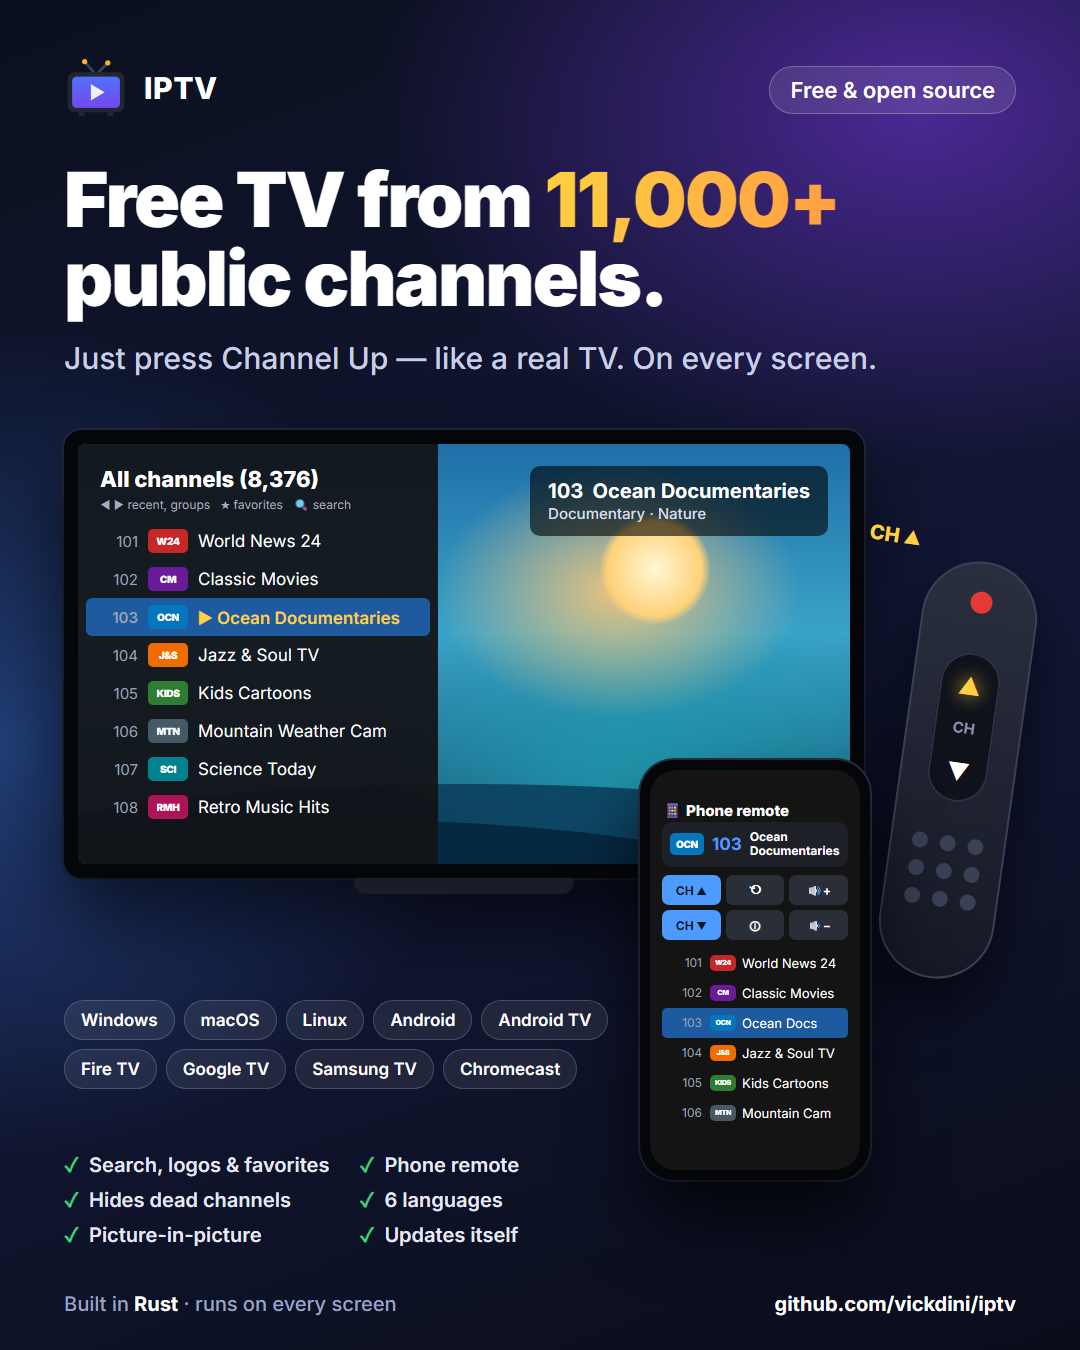
\includegraphics[width=0.52\textwidth]{../images/iptv-overview.png}\par
  \vfill
  {\large Windows \textbullet{} macOS \textbullet{} Linux \textbullet{} Android
   \textbullet{} Android TV \& Fire TV \textbullet{} Chromecast \textbullet{} Samsung TV\par}
  \vspace{0.5cm}
  {\color{dim} #2 \version{} \textbullet{} \url{https://github.com/vickdini/iptv}\par}
\end{titlepage}
\tableofcontents
\thispagestyle{fancy}}


\begin{document}
\cover{Regardez des chaînes de télévision gratuites et zappez comme sur un téléviseur}{Version}

% ------------------------------------------------------------------ intro
\section{À propos d'IPTV}

IPTV lit les chaînes de télévision gratuites et librement référencées que
rassemble le projet \emph{iptv-org} (plus de 10\,000) et vous permet de
passer de l'une à l'autre comme sur un téléviseur~: chaîne suivante et
précédente, numéros de chaînes, favoris et groupes comme Infos, Films ou
Sport.

\begin{itemize}
  \item \textbf{Toujours à jour.} La liste des chaînes est actualisée à
        chaque démarrage, et l'application se met à jour d'elle-même quand
        une nouvelle version sort.
  \item \textbf{Seulement des chaînes qui marchent.} Les chaînes hors ligne
        sont masquées automatiquement~: le zapping ne s'arrête jamais sur un
        écran noir.
  \item \textbf{Trouvez vite vos chaînes.} Cherchez par nom, reconnaissez
        chaque chaîne à son logo, revenez aux chaînes regardées récemment ou
        n'affichez que les pays et les langues qui vous intéressent.
  \item \textbf{Votre langue.} IPTV parle français, anglais, italien,
        espagnol, allemand et portugais, et suit la langue de votre appareil.
        Sur les chaînes qui les diffusent, choisissez la langue audio et
        activez les sous-titres.
  \item \textbf{Télécommande sur téléphone.} Pilotez la télévision ou
        l'ordinateur depuis le navigateur de votre téléphone
        (section~\ref{sec:remote}).
\end{itemize}

Chaque téléchargement contient tout le nécessaire~: il n'y a rien d'autre à
installer. Tous les téléchargements se trouvent sur la page des versions~:

\begin{center}
  \download
\end{center}

\note{\textbf{Avertissement.} IPTV n'héberge ni ne fournit aucune vidéo~: il
charge seulement une liste publique publiée par le projet iptv-org. Ne
regardez que ce que la loi de votre pays vous autorise à regarder.}

% ------------------------------------------------------------------ Windows
\section{Windows}
\label{sec:windows}

\subsection{Installation}
\begin{enumerate}
  \item Téléchargez \texttt{IPTV-Setup-\textless version\textgreater.exe}
        depuis la page des versions et ouvrez-le.
  \item Si Windows affiche \menu{Windows a protégé votre ordinateur},
        cliquez sur \menu{Informations complémentaires} puis sur
        \menu{Exécuter quand même}.
  \item Suivez le programme d'installation. Il ne demande pas de droits
        d'administrateur et ajoute un raccourci dans le menu Démarrer (et une
        icône sur le bureau, si vous le souhaitez).
\end{enumerate}
IPTV s'ouvre en plein cadre et commence aussitôt la lecture. Pour le
désinstaller, passez par \menu{Paramètres \textrightarrow{} Applications}.

\subsection{Touches}
\label{sec:keys}
Ces touches fonctionnent sur tous les ordinateurs~: Windows, macOS et Linux.

\rowcolors{2}{gray!8}{white}
\begin{xltabular}{\linewidth}{@{}KX@{}}
\keyshead{Touche}{Action}
\key{$\uparrow$} \key{$\downarrow$}, \key{PgPréc} \key{PgSuiv}, molette & chaîne suivante / précédente \\
\key{0}--\key{9}, puis attendre ou \key{Entrée} & aller à un numéro de chaîne \\
\key{Retour arrière} & revenir à la chaîne précédente \\
\key{$\leftarrow$} \key{$\rightarrow$}, \key{m} & baisser / monter le volume, couper le son \\
\key{l}, \key{Tab} ou clic droit & ouvrir / fermer la liste des chaînes \\
\key{/} ou \key{Ctrl}+\key{F} & rechercher une chaîne par son nom \\
\key{c} & choisir des pays et des langues \\
\key{g} / \key{G} & chaînes regardées récemment, puis les groupes (Infos, Films\ldots) \\
\key{s} / \key{S} & ajouter ou retirer un favori / zapper seulement entre les favoris \\
\key{a} / \key{t} & langue audio suivante / sous-titres suivants (puis désactivés) \\
\key{r} & télécommande sur téléphone~: afficher le code QR \\
\key{E} / \key{I} & exporter / importer les favoris (dossier Téléchargements) \\
\key{i} & informations sur la chaîne \\
\key{f}, double-clic & plein écran (\key{Échap} pour en sortir) \\
\key{p} & image dans l'image~: une deuxième chaîne, en petit, dans le coin inférieur droit \\
\key{[} / \key{]} & chaîne précédente / suivante de la petite image \\
\key{x}, clic sur la petite image & échanger les deux chaînes \\
\key{Espace} & pause \\
\key{h}, \key{?} ou \key{F1} & aide à l'écran \\
\key{q} & quitter \\
\bottomrule
\end{xltabular}

\subsection{La liste des chaînes}
Appuyez sur \key{l} pour ouvrir à gauche une liste déroulante des chaînes,
avec leurs logos~; la vidéo continue à côté. Faites défiler avec la molette
et cliquez sur une chaîne pour la regarder. Commencez à taper (ou appuyez sur
\key{/}) pour chercher~: les accents et les majuscules n'ont pas
d'importance. \key{Échap} ferme la liste. Appuyez sur \key{g} pour les
chaînes regardées récemment, de la plus récente à la plus ancienne.

\subsection{Pays et langues}
Appuyez sur \key{c}, tapez pour trouver un pays ou une langue, puis appuyez
sur \key{Entrée} pour le cocher~; \key{Tab} passe d'une liste à l'autre.
Ensuite, IPTV n'affiche que les chaînes des pays cochés ou dans les langues
cochées, jusqu'à ce que vous effaciez le choix (\key{Suppr}, ou la ligne
\emph{Effacer tous les filtres}).

\subsection{Langue audio et sous-titres}
Quand une chaîne propose plusieurs langues audio ou des sous-titres, une note
en bas de l'écran l'indique. Appuyez sur \key{a} pour la langue audio
suivante et sur \key{t} pour les sous-titres suivants (et enfin
\emph{désactivés}). IPTV retient la langue et l'utilise sur toutes les autres
chaînes qui la proposent.

\subsection{Langue et mises à jour}
IPTV utilise la langue du système. À chaque démarrage, il vérifie s'il existe
une nouvelle version~; si oui, il l'installe sans rien demander et redémarre
de lui-même au bout de quelques secondes.

% ------------------------------------------------------------------ macOS
\section{macOS}

\subsection{Installation}
\begin{enumerate}
  \item Vérifiez la puce de votre Mac~: \menu{menu Pomme \textrightarrow{} À
        propos de ce Mac}.
  \item Téléchargez l'image disque correspondante depuis la page des
        versions~:
  \begin{itemize}
    \item Apple silicon (M1, M2, M3, M4\ldots)~:
          \texttt{IPTV-\textless version\textgreater-macOS-arm64.dmg}
    \item Intel~: \texttt{IPTV-\textless version\textgreater-macOS-x86\_64.dmg}
  \end{itemize}
  \item Ouvrez-la et faites glisser \textbf{IPTV} sur \textbf{Applications}.
\end{enumerate}

\subsection{Premier lancement}
IPTV n'est pas notarié par Apple~: la première fois, macOS refuse de
l'ouvrir. Il ne faut le faire qu'une fois~:
\begin{enumerate}
  \item Ouvrez IPTV depuis Applications. Quand macOS indique qu'il ne peut
        pas être ouvert, cliquez sur \menu{OK}.
  \item Ouvrez \menu{Réglages Système \textrightarrow{} Confidentialité et
        sécurité}, descendez jusqu'à \menu{«~IPTV~» a été bloqué\ldots} et
        cliquez sur \menu{Ouvrir quand même}, puis confirmez.
\end{enumerate}

\subsection{Utilisation}
IPTV utilise les mêmes touches que sous Windows (section~\ref{sec:keys}).
Dans le Dock, il apparaît sous le nom \textbf{IPTV} pendant la lecture d'une
chaîne.

\tip{Gardez IPTV dans le dossier Applications~: lancé depuis l'image disque ou
depuis Téléchargements, macOS l'exécute depuis une copie en lecture seule et
il ne peut pas se mettre à jour.}

% ------------------------------------------------------------------ Linux
\section{Linux}

\subsection{Installation}
Téléchargez \texttt{IPTV-\textless version\textgreater-x86\_64.AppImage}
depuis la page des versions. C'est un seul fichier qui contient tout.
Rendez-le exécutable et lancez-le~:
\begin{center}
\begin{minipage}{0.8\linewidth}
\small\ttfamily chmod +x IPTV-*-x86\_64.AppImage\\
./IPTV-*-x86\_64.AppImage
\end{minipage}
\end{center}
Vous pouvez aussi, dans un gestionnaire de fichiers, ouvrir
\menu{Propriétés \textrightarrow{} Permissions}, cocher \menu{Autoriser
l'exécution du fichier comme un programme}, puis double-cliquer dessus.

Il fonctionne sur les PC 64 bits avec un Linux de 2022 ou plus récent
(Ubuntu 22.04, Debian 12, Fedora 36, Linux Mint 21 et suivants).

\tip{Des outils comme \emph{Gear Lever} ou \emph{AppImageLauncher} ajoutent
IPTV au menu des applications. Si l'AppImage signale qu'il manque FUSE,
lancez-le avec \texttt{-{}-appimage-extract-and-run}.}

\subsection{Utilisation}
IPTV utilise les mêmes touches que sous Windows (section~\ref{sec:keys}). Il
se met à jour en remplaçant le fichier AppImage~: gardez-le dans un dossier
où vous pouvez écrire (votre dossier personnel, par exemple).

% ------------------------------------------------------------------ Android
\section{Téléphones et tablettes Android}

\subsection{Installation}
\begin{enumerate}
  \item Sur le téléphone, téléchargez
        \texttt{IPTV-\textless version\textgreater.apk} depuis la page des
        versions et ouvrez-le.
  \item Android demande une fois d'autoriser l'installation d'applications
        depuis le navigateur ou le gestionnaire de fichiers~: autorisez-la,
        puis touchez \menu{Installer}.
  \item IPTV n'est pas sur Google Play~: Play Protect peut signaler un
        développeur inconnu. Choisissez \menu{Installer quand même}.
\end{enumerate}
Vous pouvez aussi l'installer avec \emph{Obtainium}, qui tient les
applications à jour directement depuis leur page des versions.

\subsection{Gestes}
\rowcolors{2}{gray!8}{white}
\begin{xltabular}{\linewidth}{@{}KX@{}}
\keyshead{Geste}{Action}
balayer vers le haut / le bas & chaîne suivante / précédente \\
toucher & ouvrir / fermer la liste des chaînes \\
toucher deux fois & revenir à la chaîne précédente \\
appui long & informations sur la chaîne \\
\bottomrule
\end{xltabular}

\subsection{Deux chaînes à la fois}
Tenez le téléphone ou la tablette à la verticale et l'écran se partage en
deux, une chaîne au-dessus de l'autre. Touchez une moitié pour l'entendre~:
un fin cadre bleu la signale, et la liste des chaînes et la télécommande sur
téléphone agissent sur elle. Balayez une moitié vers le haut ou le bas pour
changer sa chaîne. Remettez l'appareil à l'horizontale pour une seule chaîne.

\subsection{Image dans l'image}
Quittez l'application pendant que vous regardez (bouton Accueil, ou balayez
vers le haut depuis le bas de l'écran)~: la chaîne continue dans une petite
fenêtre au-dessus de vos autres applications, avec des boutons pour changer
de chaîne. Touchez la fenêtre pour revenir à IPTV, ou faites-la glisser hors
de l'écran pour la fermer. Nécessite Android 8 ou plus récent.

Écran éteint ou téléphone verrouillé, la chaîne continue~: l'écran de
verrouillage l'affiche, avec des boutons pour changer de chaîne ou arrêter.

\subsection{La liste des chaînes}
Touchez l'écran pour l'ouvrir. Touchez une chaîne pour la regarder~; un appui
long l'ajoute aux favoris ou l'en retire. Les boutons du haut~:
\begin{itemize}
  \item Champ de \textbf{recherche}~: tapez une partie du nom d'une chaîne.
  \item Flèches $\blacktriangleleft$\,$\blacktriangleright$~: groupe précédent
        / suivant.
  \item \textbf{Horloge}~: les chaînes regardées récemment.
  \item $\bigstar$~: favoris seulement. Un appui long permet d'enregistrer
        vos favoris dans un fichier ou de les ajouter depuis un fichier.
  \item \textbf{Globe}~: choisir des pays et des langues.
  \item \textbf{Sous-titres} (seulement sur les chaînes qui proposent un
        choix)~: langue audio et sous-titres.
  \item \textbf{Télécommande sur téléphone}~: piloter IPTV depuis un autre
        téléphone (section~\ref{sec:remote}).
  \item \textbf{Caster}~: lire sur un Chromecast
        (section~\ref{sec:chromecast}).
  \item \textbf{Quitter}~: ferme IPTV (et arrête la diffusion).
\end{itemize}

\subsection{Langue et mises à jour}
IPTV utilise la langue du téléphone. Il vérifie au démarrage s'il existe une
nouvelle version. La première fois, Android demande d'autoriser IPTV à
installer des applications~; ensuite, les mises à jour s'installent avec au
plus une confirmation.

% ------------------------------------------------------------------ Android TV
\section{Android TV, Google TV et Fire TV}

La même application fonctionne sur les appareils TV et se pilote avec la
télécommande. Les boutiques TV ne la proposent pas~: elle s'installe une
fois avec l'application gratuite \emph{Downloader}.

\begin{itemize}
  \item \textbf{Fire TV / Fire TV Stick~:} installez \emph{Downloader} depuis
        la boutique Amazon. Ouvrez ensuite \menu{Paramètres \textrightarrow{}
        Ma Fire TV \textrightarrow{} Options pour les développeurs
        \textrightarrow{} Installer des applis inconnues} et activez
        Downloader.
  \item \textbf{Google TV, Chromecast avec Google TV, Android TV~:} installez
        \emph{Downloader} depuis le Play Store et autorisez-le dans
        \menu{Paramètres \textrightarrow{} Applications \textrightarrow{}
        Sécurité et restrictions \textrightarrow{} Sources inconnues}.
\end{itemize}
Dans Downloader, saisissez
\begin{center}
  \download
\end{center}
puis téléchargez \texttt{IPTV-\textless version\textgreater.apk} et
installez-le. IPTV apparaît ensuite parmi les applications de la télévision.

\subsection{Télécommande}
\rowcolors{2}{gray!8}{white}
\begin{xltabular}{\linewidth}{@{}KX@{}}
\keyshead{Bouton}{Action}
Haut / Bas, Chaîne +/$-$, Avance / Retour rapide & chaîne suivante / précédente \\
OK, Lecture/Pause, Menu & ouvrir / fermer la liste des chaînes \\
Gauche / Droite & chaînes regardées récemment, puis les groupes \\
0--9 (si la télécommande en a) & aller à un numéro de chaîne \\
Retour & fermer la liste \\
Info & informations sur la chaîne \\
Touches Audio / CC (s'il y en a) & langue audio / sous-titres suivants \\
\bottomrule
\end{xltabular}

Dans la liste des chaînes, appuyez sur Haut sur la première chaîne pour
atteindre le champ de recherche. Les boutons en haut de la liste choisissent
les pays et les langues, l'audio et les sous-titres, et ouvrent la
télécommande sur téléphone.

\tip{La plupart de ces télécommandes n'ont pas de touches numériques~: la
télécommande sur téléphone (section~\ref{sec:remote}) est le moyen le plus
rapide de choisir une chaîne.}

% ------------------------------------------------------------------ Chromecast
\section{Chromecast}
\label{sec:chromecast}

Les anciens Chromecast (la simple clé sans télécommande) ne peuvent pas
installer d'applications. Castez vers eux depuis l'application Android~:
\begin{enumerate}
  \item Vérifiez que le téléphone et le Chromecast sont sur le même Wi-Fi.
  \item Ouvrez la liste des chaînes dans IPTV, touchez le bouton
        \textbf{Caster} et choisissez votre Chromecast.
  \item Zappez sur le téléphone comme d'habitude~: la télévision suit.
\end{enumerate}
Certaines chaînes ne peuvent pas être castées, car leurs serveurs ne le
permettent pas~; IPTV les saute automatiquement.

% ------------------------------------------------------------------ Samsung
\section{Téléviseurs connectés Samsung}

IPTV fonctionne sur les téléviseurs Samsung à partir de 2019. Samsung ne
permet d'installer des applications absentes de sa boutique que depuis un
ordinateur, avec le téléviseur en \emph{mode développeur}. La configuration
se fait une seule fois, depuis un PC Windows sur le même Wi-Fi que le
téléviseur.

\subsection{Installation}
\begin{enumerate}
  \item Sur le PC, installez depuis \url{https://developer.tizen.org} les
        outils en ligne de commande de \emph{Tizen Studio}. Dans son Package
        Manager, installez \emph{Samsung Certificate Extension} et \emph{TV
        Extensions Tools} (onglet \menu{Extension SDK}).
  \item Sur le téléviseur, ouvrez \menu{Applications} et tapez
        \key{1}\key{2}\key{3}\key{4}\key{5} avec la télécommande. Activez le
        \menu{mode développeur}, saisissez l'adresse IP du PC et redémarrez le
        téléviseur.
  \item Téléchargez \texttt{IPTV-Samsung-TV-\textless version\textgreater.zip}
        depuis la page des versions et décompressez-le.
  \item Trouvez l'adresse IP du téléviseur (\menu{Paramètres
        \textrightarrow{} Général \textrightarrow{} Réseau \textrightarrow{}
        État du réseau}) et exécutez, dans le dossier décompressé~:
\begin{center}
\begin{minipage}{0.92\linewidth}
\small\ttfamily powershell -ExecutionPolicy Bypass -File install-on-tv.ps1 -TvIp 192.168.1.4
\end{minipage}
\end{center}
        La première fois, il explique comment créer le certificat Samsung
        gratuit (avec un compte Samsung). Relancez-le ensuite~: il installe
        IPTV, qui apparaît alors dans les Applications du téléviseur.
\end{enumerate}
Ensuite, IPTV se met à jour tout seul~: inutile de refaire la configuration
pour les nouvelles versions. Il utilise la langue du téléviseur.

\subsection{Télécommande}
\rowcolors{2}{gray!8}{white}
\begin{xltabular}{\linewidth}{@{}KX@{}}
\keyshead{Bouton}{Action}
Haut / Bas, CH + / CH $-$ & chaîne suivante / précédente \\
0--9 & aller à un numéro de chaîne \\
OK & liste des chaînes (dans la liste~: regarder la chaîne sélectionnée) \\
Gauche / Droite & chaînes regardées récemment, puis les groupes \\
PRE-CH & revenir à la chaîne précédente \\
INFO & informations sur la chaîne \\
\colorkey{tvred}{Rouge} & ajouter ou retirer un favori \\
\colorkey{tvgreen}{Vert} & favoris seulement \\
\colorkey{tvyellow}{Jaune} & menu langue audio et sous-titres \\
\colorkey{tvyellow}{Jaune} dans la liste & choisir des pays et des langues \\
\colorkey{tvblue}{Bleu} & rechercher une chaîne par son nom \\
Retour & fermer la liste, ou quitter IPTV \\
\bottomrule
\end{xltabular}

\note{La télécommande sur téléphone (section~\ref{sec:remote}) n'est pas
encore disponible sur les téléviseurs Samsung. L'application gratuite
\emph{SmartThings} sert de télécommande sur téléphone pour les touches de
base.}

% ------------------------------------------------------------------ remote
\section{Télécommande sur téléphone}
\label{sec:remote}

Pilotez IPTV depuis votre téléphone, Android ou iPhone, sans rien installer.
Vous pouvez parcourir et rechercher toutes les chaînes et en toucher une pour
la regarder~; la télécommande propose aussi les favoris, les chaînes
regardées récemment, chaîne suivante / précédente, le volume, la langue
audio et les sous-titres. Elle fonctionne avec IPTV sur un ordinateur et sur
Android TV, Google TV et Fire TV, et parle la langue de votre téléphone.

\begin{enumerate}
  \item Sur un ordinateur, appuyez sur \key{r}. Sur Android TV, Google TV ou
        Fire TV, ouvrez la liste des chaînes et choisissez le bouton
        \textbf{télécommande sur téléphone}. Un code QR apparaît.
  \item Scannez-le avec l'appareil photo du téléphone. Le téléphone doit être
        sur le même Wi-Fi. Sans appareil photo, ouvrez dans le navigateur du
        téléphone l'adresse affichée à l'écran et saisissez le code.
  \item La télécommande s'ouvre dans le navigateur du téléphone. Ajoutez-la à
        l'écran d'accueil ou à vos favoris~: désormais, elle se connecte
        d'elle-même dès qu'IPTV est lancé.
\end{enumerate}

Pour transférer vos favoris vers un autre téléviseur ou ordinateur, utilisez
\textbf{Enregistrer sur le téléphone} en bas de la page de la télécommande,
puis \textbf{Ajouter depuis un fichier} dans la télécommande de l'autre
appareil. Les favoris sont ajoutés, jamais supprimés. Sur un ordinateur, vous
pouvez aussi appuyer sur \key{E} (enregistrer dans le dossier
Téléchargements) et sur \key{I} (ajouter depuis ce dossier)~; sur les
téléphones et tablettes Android, faites un appui long sur le bouton
$\bigstar$.

\note{La première fois, Windows (et macOS, si son pare-feu est activé)
demande si IPTV peut utiliser le réseau~: autorisez-le sur les réseaux
\textbf{privés}, sinon les téléphones ne pourront pas se connecter. Seuls les
téléphones qui connaissent le code peuvent piloter IPTV.}

% ------------------------------------------------------------------ help
\section{Dépannage}

\begin{description}[style=nextline, leftmargin=0pt, itemsep=6pt]
  \item[Une chaîne ne se lance pas.] Beaucoup de chaînes gratuites cessent
        d'émettre ou ne fonctionnent que dans certains pays. IPTV les masque
        et passe tout seul à la suivante~; changez simplement de chaîne.
  \item[La liste semble plus courte qu'avant.] Vérifiez si des pays ou des
        langues sont choisis (\key{c} sur un ordinateur, le bouton globe sur
        Android, \colorkey{tvyellow}{Jaune} dans la liste sur les téléviseurs
        Samsung) et effacez-les.
  \item[La télécommande sur téléphone ne se connecte pas.] Vérifiez que le
        téléphone est sur le même Wi-Fi (et non en données mobiles) et que le
        pare-feu de l'ordinateur autorise IPTV sur les réseaux privés.
  \item[Des sous-titres sont listés mais rien n'apparaît.] Certaines chaînes
        annoncent des sous-titres qu'elles n'envoient pas vraiment. IPTV n'y
        est pour rien.
  \item[IPTV n'est pas dans la bonne langue.] Il suit la langue de
        l'appareil (sur un ordinateur, celle du système). Les noms des
        chaînes, des groupes et des pays viennent de la liste et sont
        toujours en anglais.
  \item[Autre chose~?] Signalez-le sur
        \url{https://github.com/vickdini/iptv/issues}.
\end{description}

\vfill
{\small\color{dim} IPTV est un logiciel libre sous licence GNU General
Public License, version 3 ou ultérieure. Son code source se trouve sur
\url{https://github.com/vickdini/iptv}.\par}

\end{document}
